
\section{Integralregning og arealer}
Forklar begreberne stamfunktion og bestemt integral.
\subsection{Bevis af at arealfunktionen er stamfunktionen}

\begin{proofw}
    
Betragt følgende skitse:

\begin{figure}[h]
    \centering
    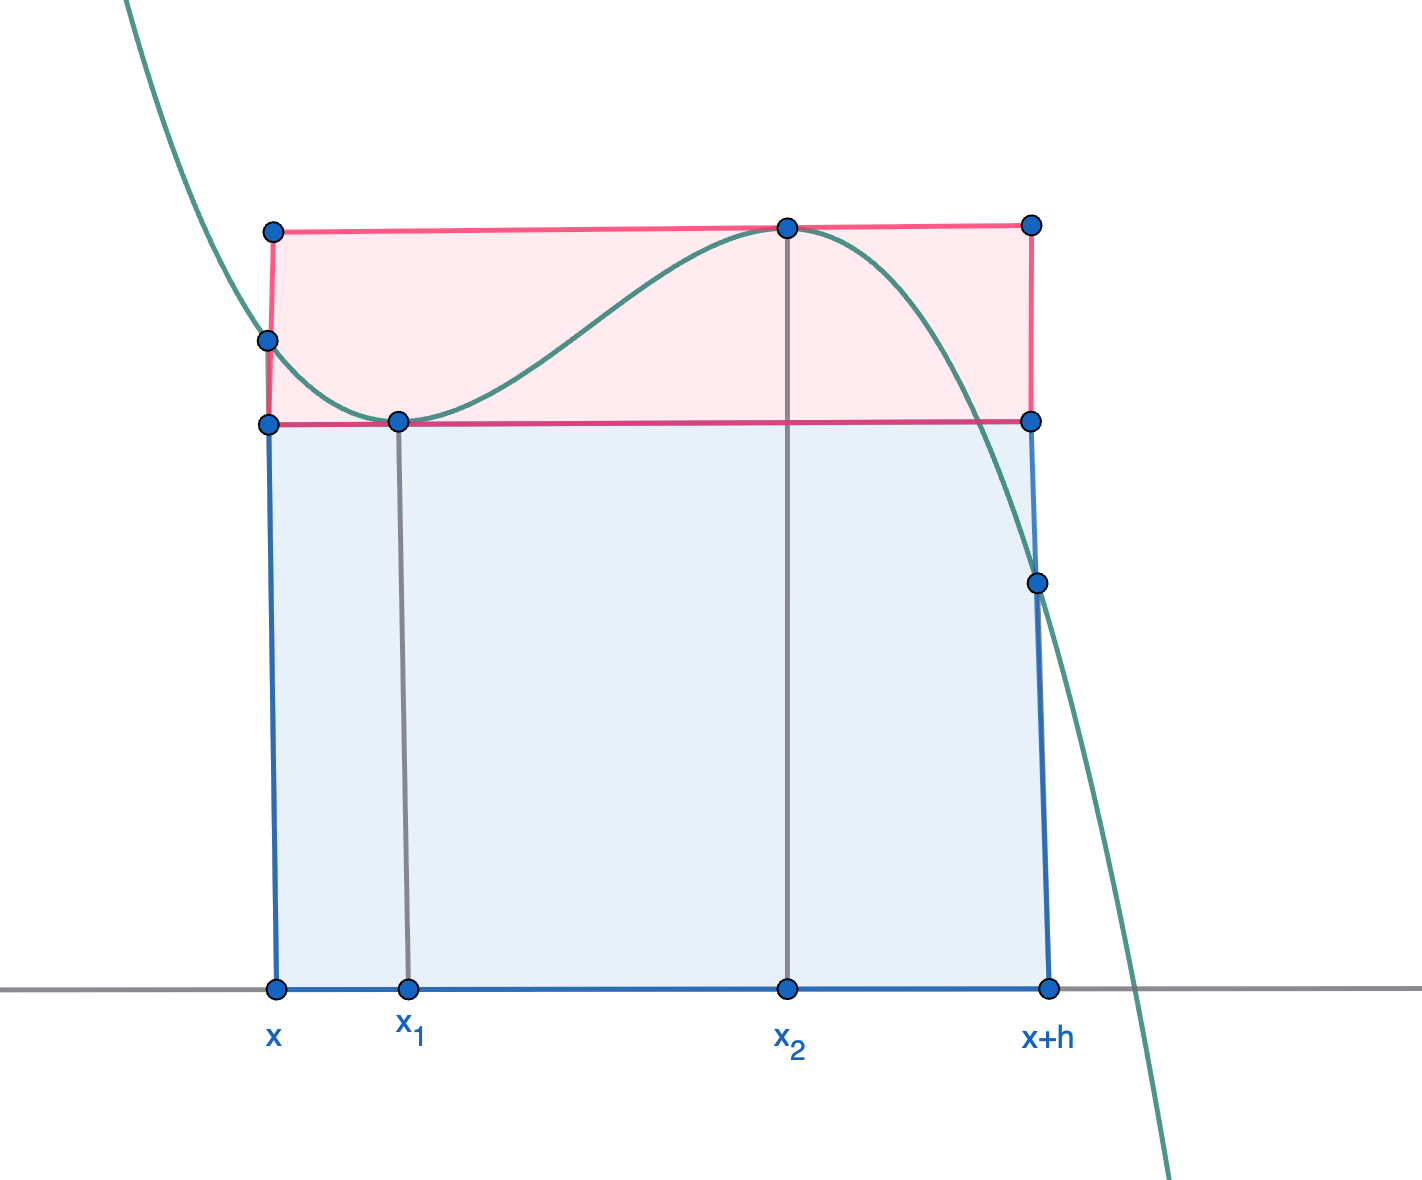
\includegraphics[scale=0.3]{skitser/areal_funktion.png}
\end{figure}

Vi betragter et udsnit af en funktion,
hvor vi ønsker at finde arealet mellem funktionen og $x$-aksen.
Vi antager, at en funktion $A(x)$ giver arealet under grafen indtil $x$-værdien,
og at arealet under grafen på udsnittet ville være givet ved:

$$
    A_{graf}=A(x+h)-A(x)
$$

I udsnittet har vi markeret et interval $x$ til $x+h$,
indenfor dette interval er der et lokalt minimum og maksimum for funktionen.
Arealet under grafen skal være større end eller lig arealet af den blå kasse,
som har længde $h$ og højde $f(x_1)$.
Og arealet skal også være mindre eller lig
arealet af den blå kasse + den røde kasse,
hvilket er den kasse, som har længde $h$ og højde $f(x_2)$.
Derfor kan vi opstille følgende ulighed, som vi kan regne med:

$$
    f(x_1) \cdot h \leq A(x+h)-A(x)
    \leq f(x_2) \cdot h
$$

Først dividerer vi med $h$ på alle sider:

$$
    f(x_1) \leq \frac{A(x+h)-A(x)}{h} \leq f(x_2)
$$

Og så lader vi $h \rightarrow 0$ og deraf:

\begin{align*}
    x_1 &\rightarrow x \\
    x_2 &\rightarrow x \\
    f(x_1) &\rightarrow f(x) \\
    f(x_2) &\rightarrow f(x) \\
    \frac{A(x+h)-A(x)}{h} &\rightarrow A'(x)
\end{align*}

Dette vil sige, at:

$$
    f(x) \leq A'(x) \leq f(x)
$$

Så:
$$
    f(x) = A'(x)
$$

Altså er arealfunktionen af en graf en stamfunktion til funktionen.

\end{proofw}
